\documentclass[footinbib,amsmath,amssymb,%
superscriptaddress,twocolumn]{revtex4}
\usepackage{graphicx,amsmath}
\usepackage{color}
\usepackage{siunitx}
\begin{document}


\title{Supplementary Informations to:\\Gelation as condensation frustrated by hydrodynamics and mechanical tension}
\author{Hideyo Tsurusawa}
\affiliation{ {Institute of Industrial Science, University of Tokyo, 4-6-1 Komaba, Meguro-ku, Tokyo 153-8505, Japan} }
%\thanks{These authors contributed equally to this work}
\author{Mathieu Leocmach}
\affiliation{Univ Lyon, Université Claude Bernard Lyon 1, CNRS, Institut Lumière Matière, F-69622, VILLEURBANNE, France}
%\thanks{These authors contributed equally to this work}
\author{Hajime Tanaka}
%\email{tanaka@iis.u-tokyo.ac.jp}
\affiliation{ {Institute of Industrial Science, University of Tokyo, 4-6-1 Komaba, Meguro-ku, Tokyo 153-8505, Japan} }

\maketitle

\begin{figure}
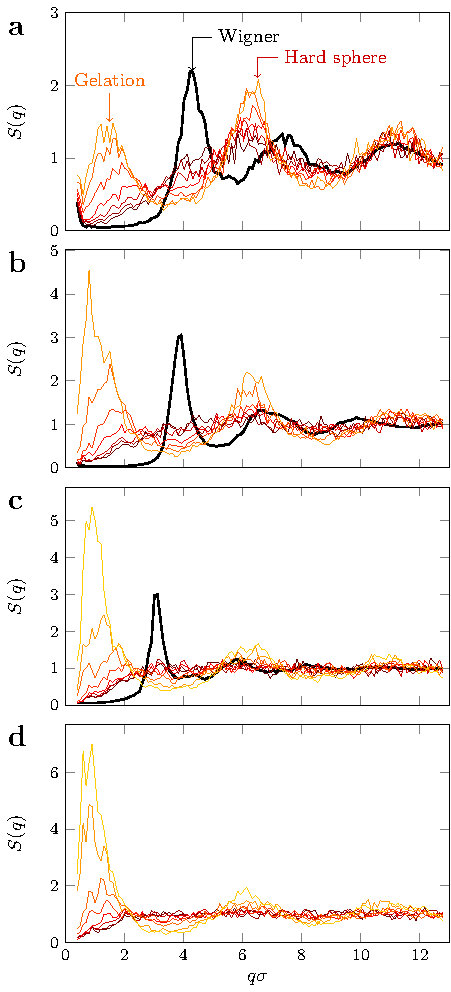
\includegraphics{figs/structure_factor.pdf}
\caption{\textbf{Structure factor evolution} in the four samples shown on Fig. 2 of the main text by decreasing volume fraction. The thick black curve corresponds to the intial wigner crystal before salt introduction (ill defined thus not shown in \textbf{d}). Thin curves from dark red to yellow are spaced by \SI{150}{\second} and display a peak corresponding to the hard sphere diameter as well as a growing peak at low $q$ inticating gelation.}
\label{fig:structure_factor}
\end{figure}

\end{document}